
\subsubsection{Syntax Introduction}
For the following algorithms in section \ref{sec:scheduling}:

\textbf{Partial Systems:} A partial system $\lambda^\prime$ is defined as a system that processes a specific set of archetypes, instead of its requirements. The following is the syntax definition:

\begin{equation}
    \lambda^\prime := \{a_1,a_2,\ldots,a_n\} \in \mathcal{P}(A) : \lambda[a_1][a_2]\ldots[a_n]
    \label{eq:partial_lambda}
\end{equation}

These $\lambda^\prime$ systems will later be used to express what archetypes are concurrently computable with respect to another system.

\textbf{Set Symmetric Difference:} $\Delta$ used in the following algorithms is defined as the symmetric difference: 
$$x_1 \Delta x_2 := (x \cup x_1) \setminus (x \cap x_1)$$


\subsubsection{Partitioning Algorithm}
\label{alg:part}
The following algorithm presented in the paper is used to determine what systems are parallelizable based on the entity FSM introduced in section \ref{sec:fsm_arc}. 

\begin{enumerate}
    \item Initiate sets $par, seq$ such that they will contain tuples of type $(\lambda, \lambda^\prime)$
    \item Initiate vector $v_1$ that will contain tuples of the type $(\lambda \in \Lambda, x \subseteq \mathcal{P}(A))$
    \item For each $\lambda \in \Lambda$, do the following steps 4-5:
    \item Construct the set $x = \{ \forall a \in A : a \cap \lambda_{req} \not= \emptyset \}$
    \item Push to $v_1$: $(\lambda, x)$
    \item For each $(\lambda, x) \in v_1$, do the following steps 7-8:
    \item Calculate the sequential set $X_{seq} = \{ (\lambda_1, x_1 \cap x ) : (\lambda_1, x_1) \in v_1 \land \lambda_1 \not= \lambda \}$. This set contains all archetypes that appear in $\lambda_1$ relative to $\lambda$.
    \item Calculate the parallel set $X_{par} = \{ (\lambda_1, x_1 \setminus x ) : (\lambda_1, x_1) \in v_1 \land \lambda_1 \not= \lambda \}$. This set contains archetypes that are parallelizable relative to $\lambda$.
    \item Push to set $seq$ the array of values $[\forall x_0,x_1,\ldots,x_n \in X_{seq} : \lambda[x_0][x_1]\ldots[x_n]]$ interleaved with $\Lambda$ to create tuples $(\lambda, \lambda^\prime)$.
    \item Do the same as in step 9 but for the $par$ set.
\end{enumerate}

After all the steps above, the set $seq$ and $par$ contains a function $\lambda$ that, relative to $\lambda^\prime$, is parallelizable or not parallelizable depending on the set. These two sets will later be used to generate a computation graph of how to schedule the ECS.

Although the algorithm for partitioning in section \ref{alg:part} is $O(N^2)$ where $N$ is the number of archetypes, its unlikely that there will ever enough types of components and lazily loaded archetypes on the graph for it to matter in any circumstance, but it is important to still bring awareness.

% TODO: ACTUALLY DO IT
Depending on the leniency of defining $\lambda_{req}$, its possible to only ever have to do this calculation once. If all systems are defined at compile time and new systems are not allowed to be added during runtime, the computation graph will never change. The implementation in this paper allows new systems to be defined at runtime and only needs to recalculate on new archetype additions to the Entity FSM.

\subsubsection{Example Computation}
The following section is dedicated to producing the $seq$ and $par$ sets based on the entity FSM in Figure \ref{fig:graph1}. Suppose instead of $\Lambda = \emptyset$:


\textbf{Vector Production:} The first step is generating the $v_1$ vector.

\begin{align*}
    v_1[\lambda_1] &= \{ \forall a \in A : a \cup [A,C] \neq \emptyset \} & \Rightarrow &
    \quad v_1[\lambda_1] = \{[A],[AC],[AB],[ABC]\} \\
    v_1[\lambda_2] &= \{ \forall a \in A : a \cup [B,C] \neq \emptyset \} & \Rightarrow &
    \quad v_1[\lambda_2] = \{[B],[AB],[AC],[BD],[ABC]\} \\
    v_1[\lambda_3] &= \{ \forall a \in A : a \cup [D] \neq \emptyset \} & \Rightarrow &
    \quad v_1[\lambda_3] = \{[D],[BD]\}
\end{align*}

\textbf{Sequential Set:} The next step is to generate the set $X_{seq}$ for each set in $v_1$.

\begin{align*}
    \lambda_1: \quad & X_{seq} = \{v_1[\lambda_1] \cap v_1[\lambda_2], v_1[\lambda_1] \cap v_1[\lambda_3]\} & \Rightarrow & \quad X_{seq} = \{[AC][AB][ABC],[]\} \\ 
    \lambda_2: \quad & X_{seq} = \{v_1[\lambda_2] \cap v_1[\lambda_1], v_1[\lambda_2] \cap v_1[\lambda_3]\} & \Rightarrow & \quad X_{seq} = \{[AC][AB][ABC],[BD]\} \\ 
    \lambda_3: \quad & X_{seq} = \{v_1[\lambda_3] \cap v_1[\lambda_1], v_1[\lambda_3] \cap v_1[\lambda_2]\} & \Rightarrow & \quad X_{seq} = \{[],[BD]\} \\ 
\end{align*}

\textbf{Parallel Set:} With $v_1$ and $X_{seq}$ generated, apply to each context of $X_{seq}$ above the formula to generate $X_{par}$.
\begin{align*}
    \lambda_1: \quad & X_{par} = \{v_1[\lambda_1] \setminus v_1[\lambda_2], v_1[\lambda_1] \setminus v_1[\lambda_3]\} & \Rightarrow & \quad X_{par} = \{[A],[A][AC][AB][ABC]\} \\ 
    \lambda_2: \quad & X_{par} = \{v_1[\lambda_2] \setminus v_1[\lambda_1], v_1[\lambda_2] \setminus v_1[\lambda_3]\} & \Rightarrow & \quad X_{par} = \{[AC][AB][ABC],[BD]\} \\ 
    \lambda_3: \quad & X_{par} = \{v_1[\lambda_3] \setminus v_1[\lambda_1], v_1[\lambda_3] \setminus v_1[\lambda_2]\} & \Rightarrow & \quad X_{par} = \{[],[BD]\} \\ 
\end{align*}

\textbf{Construct Sequential Partial Functions}: With the $X_{seq}$ generated, apply the transformation into $seq$:
\begin{align*}
    \lambda_1: \quad & X_{\text{seq}}[\lambda_2]  \Rightarrow \quad \lambda_1[AC][AB][ABC] \\
                     & X_{\text{seq}}[\lambda_3]  \Rightarrow \quad \lambda_1[] \\ 
    \\[0.3em]
    \lambda_2: \quad & X_{\text{seq}}[\lambda_1]  \Rightarrow \quad \lambda_2[AC][AB][ABC] \\
                     & X_{\text{seq}}[\lambda_3]  \Rightarrow \quad \lambda_2[BD] \\
    \\[0.3em]
    \lambda_3: \quad & X_{\text{seq}}[\lambda_1]  \Rightarrow \quad \lambda_3[] \\
                     & X_{\text{seq}}[\lambda_2]  \Rightarrow \quad \lambda_3[BD]
\end{align*}

Note how $\lambda_1$ with respect to $\lambda_3$ contains a partial with empty archetypes. Although these archetypes are valid, since $\emptyset \in \mathcal{P}(T)$, they do nothing so implementation wise they are unimportant. Using this computation, the following is the set $seq$.

$$
\text{seq} = \left\{
\begin{array}{@{}l@{}}
    \lambda_1[\text{AC}][\text{AB}][\text{ABC}] \\ 
    \lambda_2[\text{AC}][\text{AB}][\text{ABC}], \lambda_2[\text{BD}] \\
    \lambda_3[\text{BD}]
\end{array}
\right\}
$$

\textbf{Construct Parallel Partial Functions}: With the $X_{par}$ generated, apply the transformation to $par$:
\begin{align*}
    \lambda_1: \quad & X_{\text{par}}[\lambda_2]  \Rightarrow \quad \lambda_1[A] \\
                     & X_{\text{par}}[\lambda_3]  \Rightarrow \quad \lambda_1[A][AC][AB][ABC] \\ 
    \\[0.3em]
    \lambda_2: \quad & X_{\text{par}}[\lambda_1]  \Rightarrow \quad \lambda_2[B] \\
                     & X_{\text{par}}[\lambda_3]  \Rightarrow \quad \lambda_2[B][AB][ABC][AC] \\
    \\[0.3em]
    \lambda_3: \quad & X_{\text{par}}[\lambda_1]  \Rightarrow \quad \lambda_3[D][BD] \\
                     & X_{\text{par}}[\lambda_2]  \Rightarrow \quad \lambda_3[D]
\end{align*}

Note how $|\lambda_1:X_{seq}[\lambda_3]| = |v_1[\lambda_1]|$. The fact that they are the same length means to us that with respect to $\lambda_3$, $\lambda_1$ is completely parallelizable. Finally, the set $par$ is:

$$
\text{par} = \left\{
\begin{array}{@{}l@{}}
    \lambda_1[\text{A}] \quad \lambda_1[\text{A}][\text{AC}][\text{AB}][\text{ABC}] \\ 
    \lambda_2[\text{B}] \quad \lambda_2[\text{B}][\text{AB}][\text{ABC}][\text{AC}] \\
    \lambda_3[\text{D}] \quad \lambda_3[\text{D}][\text{BD}]
\end{array}
\right\}
$$

\subsubsection{Scheduling Algorithm}
The two sets from the partitioning algorithm is all we need to schedule one tick.


\subsubsection{Computation Graphs}
Now with $par$ and $seq$, we are able to generate the computation graph for the systems. We sequentially process all partials in $seq$ first, and then spin up threads for each system. 

\begin{figure}[H]
    \centering
    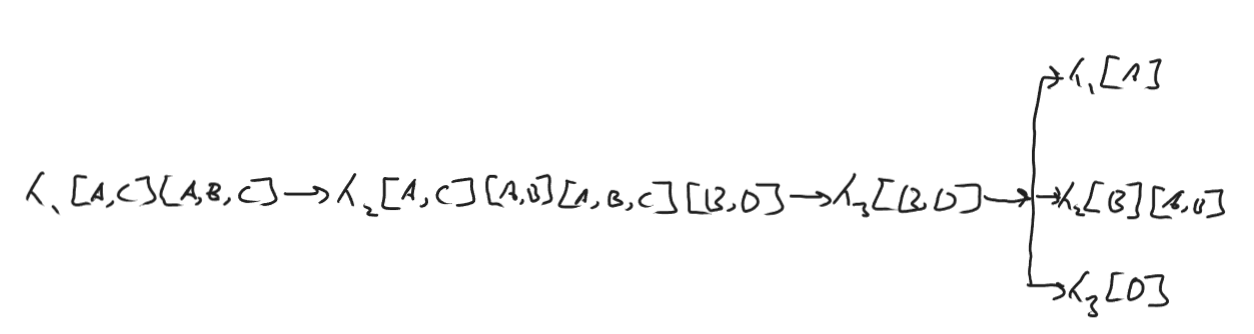
\includegraphics[width=0.5\linewidth]{resources/computation_graph.png}
    \caption{Temp Graph To Replace Later with Latex}
    \label{fig:temp1}
\end{figure}

There is a visual way to understand this algorithm. A BFS can be initiated from all starting types from the given $\lambda_{req}$ to capture the vertices in $v_1$. Then we color each vertex set with unique colors. 

\begin{figure}[H]
    \centering
    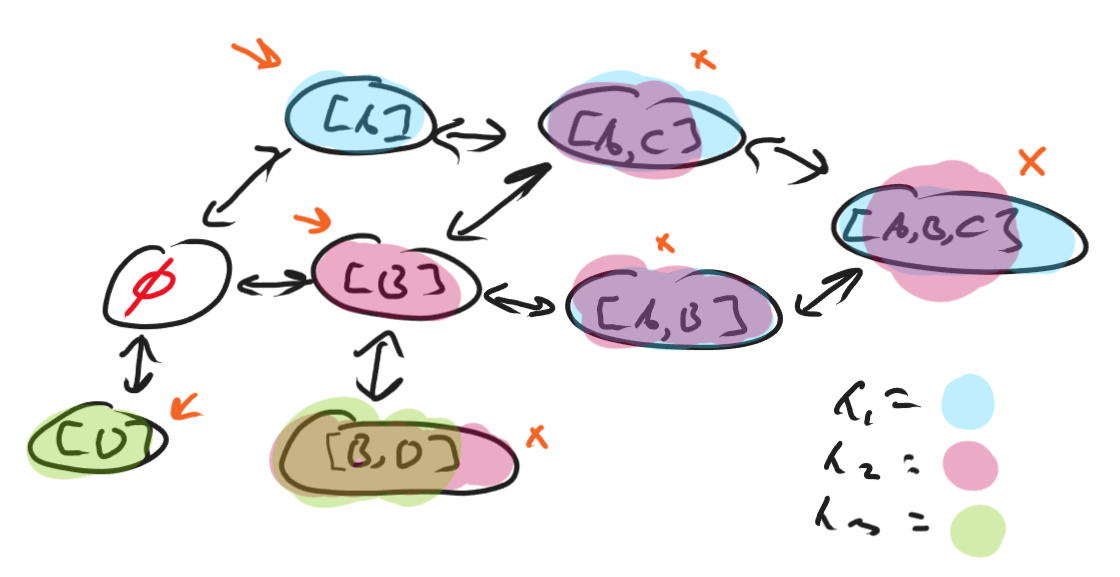
\includegraphics[width=0.5\linewidth]{resources/color_graph.png}
    \caption{Temp Graph To Replace Later with Latex}
    \label{fig:graph2}
\end{figure}

In Figure \ref{fig:graph2}, notice that all nonoverlapping colors are safe to multithread while all overlapped colors ended up in the sequential part of the computation graph.

\subsubsection{Scheduling Systems}
Now to finally scheduling the systems. Because of the hard work done in section \ref{alg:part}, the set $seq$ can just run sequentially so that will be ignored and processed on the main thread. Once those are done, we assign for each partial system $\lambda^\prime \in par$ to the next available thread in the thread pool. 
